\documentclass{report}

\usepackage{apalike}
\usepackage{graphicx}

\title{replace title}
\author{replace author}
\date{replace date}

\begin{document}
\maketitle
\tableofcontents
\listoffigures

\chapter{Introduction}

\chapter{Executive Summary}
\section{Planning}
\subsection{Approach}
\subsection{Scope}
\subsection{Objectives}
\section{Methodology}
\subsection{Information Gathering}
\subsection{System Attacks}
\section{Summary of Findings}

\chapter{Key Findings}


\section{Auction Site}
This section covers the vulnerabilities found with the user-facing auction site.
\subsection{Path Traversal}
\subsubsection{Security Implications / Risk Level}
Path traversal allows for arbitrary file read across the system, for any files readable by the apache user (www-data). This is dangerous as it could potentially leak sensitive company data, as well as user data. If combined with other vulnerabilities, such as incorrect permissions on log files, it is possible to achieve Remote Code Execution through malicious log read/write.\\
Overall, the execution of this exploit is trivial, and the repercussions are potentially serious but not disasterous. Due to this, the risk level of this exploit is evaluated to be \textbf{medium}.
\subsubsection{Cause of Vulnerability}
The vulnerability is caused by the method used to retrieve and display image files on the website. Instead of directly referencing the image file through the 'src' field on an 'img' HTML tag, a PHP script is instead used to include the file.\\ 
While using PHP include scripts may not normally be dangerous, the file name to be retrieved can be edited by the user, allowing them to easily select which file should be displayed. A lack of filter/extension whitelist makes this even more potent.
\subsubsection{Steps to Replicate}
\begin{itemize}
		\item Firstly the inspect element tool in Mozilla Firefox was used to inspect an image, revealing the image URL (Fig. 3.1).
		\item The image URL could then be opened, showing the ASCII representation of the binary content for the image file (Fig. 3.2).
		\item Finally, the URL parameter 'file' could be replaced with a file path, allowing for arbitrary file read. In this example, the ../ operator was used to go up directories until root, and then the /etc/passwd file was navigated to (Fig. 3.3).
\end{itemize}
\begin{figure}[!htb]
	\centering
	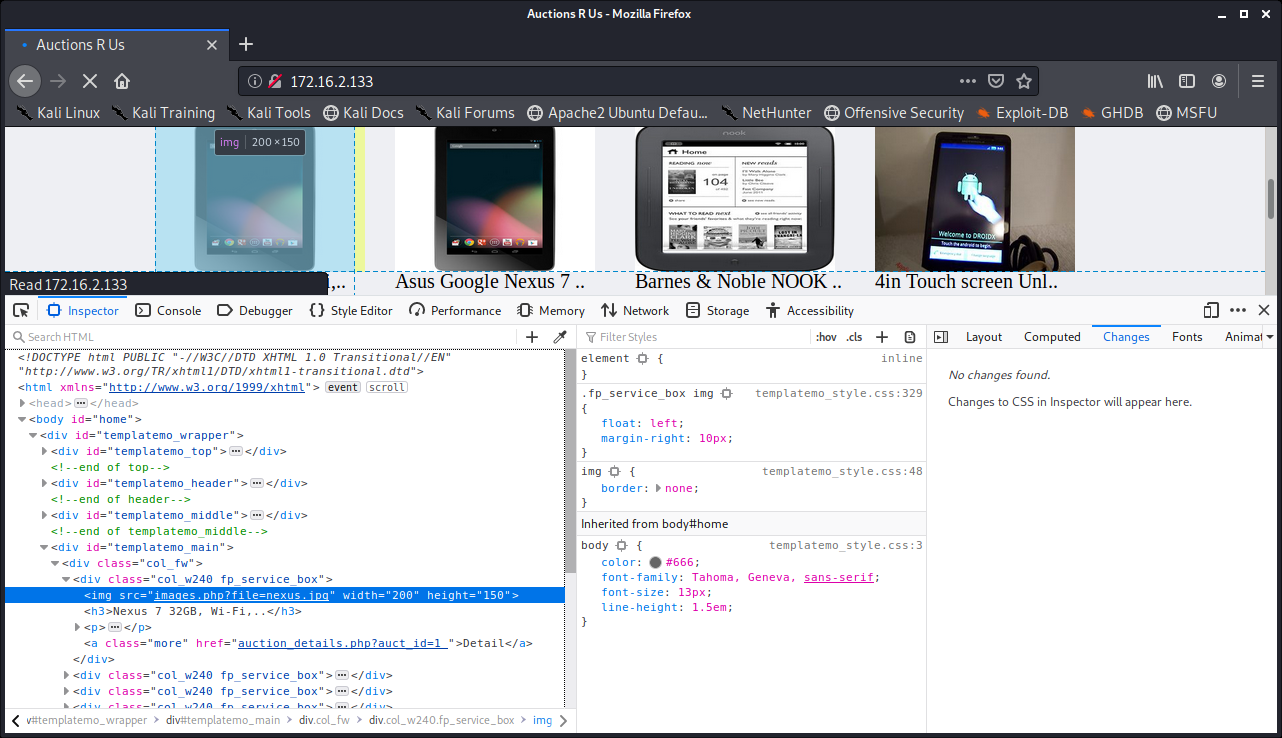
\includegraphics[scale=0.4]{img/pathtraversal1.png}
	\caption{Inspecting the image}
\end{figure}
\begin{figure}[!htb]
	\centering
	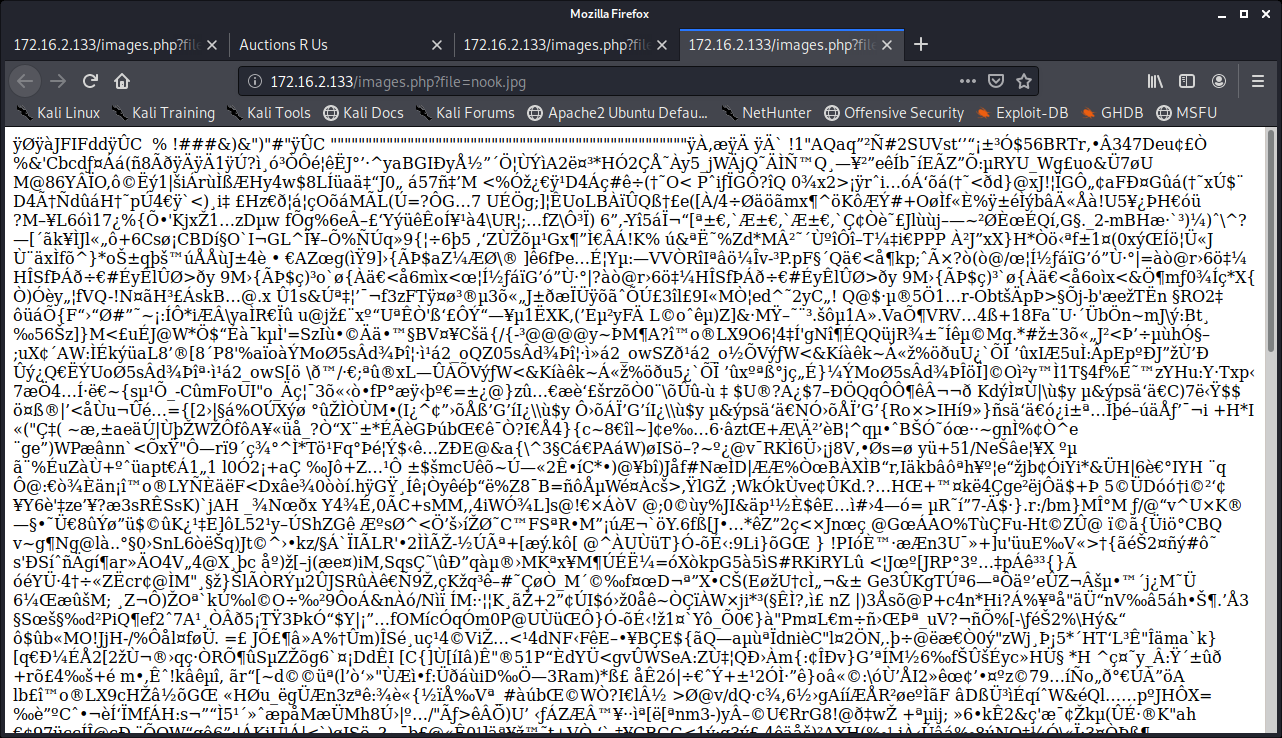
\includegraphics[scale=0.4]{img/pathtraversal2.png}
	\caption{Viewing the image contents}
\end{figure}
\begin{figure}[!htb]
	\centering
	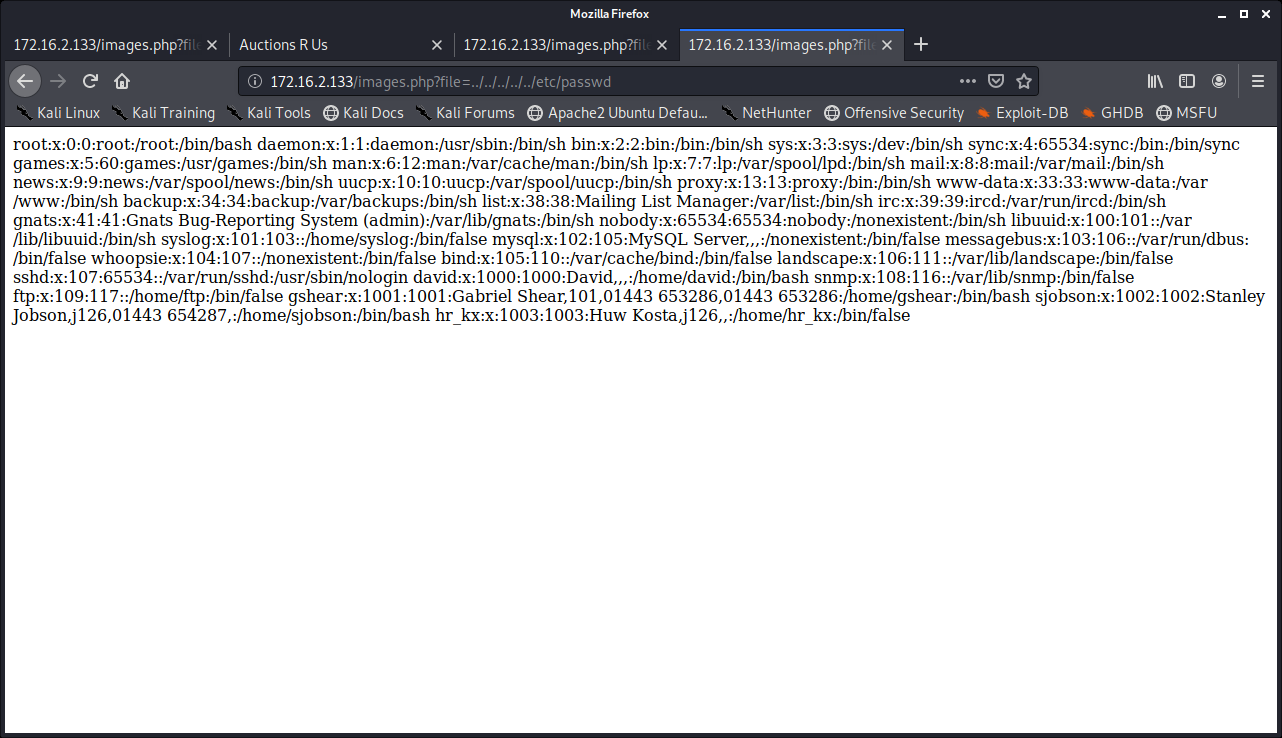
\includegraphics[scale=0.4]{img/pathtraversal3.png}
	\caption{Exploiting the file read}
\end{figure}
\pagebreak



\subsection{SQL Injection}
\subsubsection{Security Implications / Risk Level}
SQL injection is a blanket term covering any kind of unintended user control over the SQL queries interacting with a database. This can manifest in many forms, such as:
\begin{itemize}
	\item Authentication bypass, where SQL queries can be modified to bypass authentication checks such as login forms.
	\item Union injection, where the UNION keyword in SQL can be used to access data from other columns, tables, and databases.
	\item Error based injection, where SQL errors are intentionally created in order to gain information about the database.
	\item Blind injection, where queries that return TRUE or FALSE can be used to gain information about the database.
\end{itemize}
From the testing done, the website appears to be vulnerable to both authentication bypass, allowing attackers to log in to accounts, and blind injection, allowing for full read access across the database.\\
The execution of these exploits are relatively easy with the use of tools like SQLmap, and the repercussions can be very serious, allowing attackers to log in to administrator accounts as well as reading any user/auction data from the database. Due to this, the risk level of this exploit is evaluated to be \textbf{high}.
\subsubsection{Cause of Vulnerability}
SQL injection vulnerabilities are a result of allowing unsanitised user input in to SQL queries. Sanitising SQL queries involves removing any kind of dangerous character from the input, such as quotation marks (single and double) and comment tags. If this is not done, attackers are able to modify queries in specific ways to allow them to perform SQL injection.\\
One example of this would be performing an authentication bypass injection. A normal query may use a query like:
\begin{verbatim}
SELECT * FROM users WHERE username = '$inputname' AND password = 
'$inputpass';
\end{verbatim}
If an attacker enters something like ' OR 1=1\# in to the username field, the query becomes:
\begin{verbatim}
SELECT * FROM users WHERE username = '' OR 1=1#;
\end{verbatim}
Which will pick the first username from the table and sign the attacker in.
\subsubsection{Steps to Replicate}
\begin{itemize}
	\item For initial testing of SQL injection, a basic authentication bypass was used. The payload ' OR 1=1-- - was entered in to the username field (Fig. 3.4), which subsequently allowed access to the 'David' account, giving use of the admin panel as well (Fig. 3.5).
	\item For further testing, the tool SQLmap was used. This is a tool that automatically iterates through potential SQLi payloads, providing information such as DB names, table names, table data, SQL user names, and SQL version.
	\item The first test done with SQLmap was checking if it detected SQL injection. The command used for this was \begin{verbatim}sqlmap -u "http://172.16.2.133/login.php?username=qwe&
	password=qwe&Search=" --batch\end{verbatim}The results provided some information on the DB system and potential attacks it was vulnerable to (Fig. 3.6).
	\item After this, the --passwords flag was used to test for DB users and retrieve any passwords if possible. SQLmap found a DB user named "auctuser", but had no access to the users table so could not retrieve a password (Fig. 3.7).
	\item With no password found, the next step was to search for databases. The command used to do this was
\begin{verbatim}
sqlmap -u "http://172.16.2.133/login.php?username=qwe&
password=qwe&Search=" --batch --databases
\end{verbatim}
	This successfully found the databases, returning three in total (Fig. 3.8). The first was the information\_schema DB, default in all installations of MySQL. The second was the auctionsrus DB, the one likely holding all info. The last was a test DB which also comes default with MySQL.
	\item With the new information of the auctionsrs db, the --tables flag could be used to dump the table names for said DB. The command used for this was:
\begin{verbatim}
sqlmap -u "http://172.16.2.133/login.php?username=qwe&
password=qwe&Search=" --batch -D auctionsrus --tables
\end{verbatim}
	This returned two tables found in the auctionsrus DB (Fig. 3.9). One, auction\_users, was likely to contain the user data for the site, while the other, auctions, was likely to contain the auction data.
	\item Finally, the last step was to attempt to dump the data from the tables. As a proof of concept, the data from the users table was dumped using the command:
\begin{verbatim}
sqlmap -u "http://172.16.2.133/login.php?username=qwe&
password=qwe&Search=" --batch -D auctionsrus -T auction_users --dump
\end{verbatim}
	This returned the full set of user data from the auction\_users table, including usernames, MD5 hashed passwords (all cracked, with the one not displayed on the screenshot being '7331'), user IDs, and user levels (Fig. 3.10). With the dump done, the full extent of the SQL injection was explored.
\end{itemize}
\pagebreak
\begin{figure}[!htb]
	\centering
	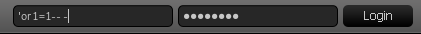
\includegraphics[scale=1]{img/sqli1.png}
	\caption{Authentication bypass SQLi}
\end{figure}
\begin{figure}[!htb]
	\centering
	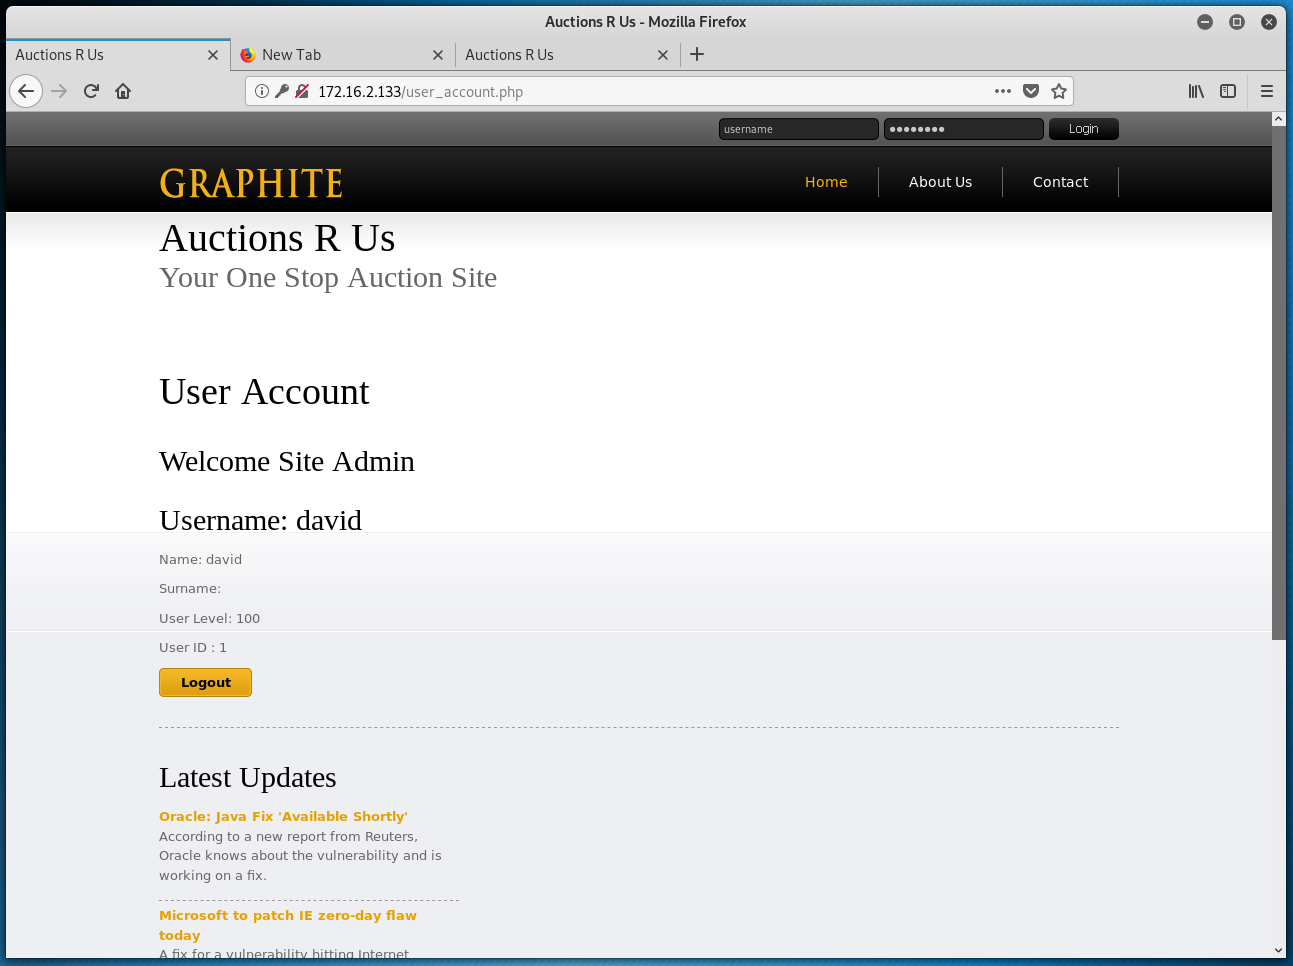
\includegraphics[scale=0.4]{img/sqli2.png}
	\caption{Admin panel access gained}
\end{figure}
\begin{figure}[!htb]
	\centering
	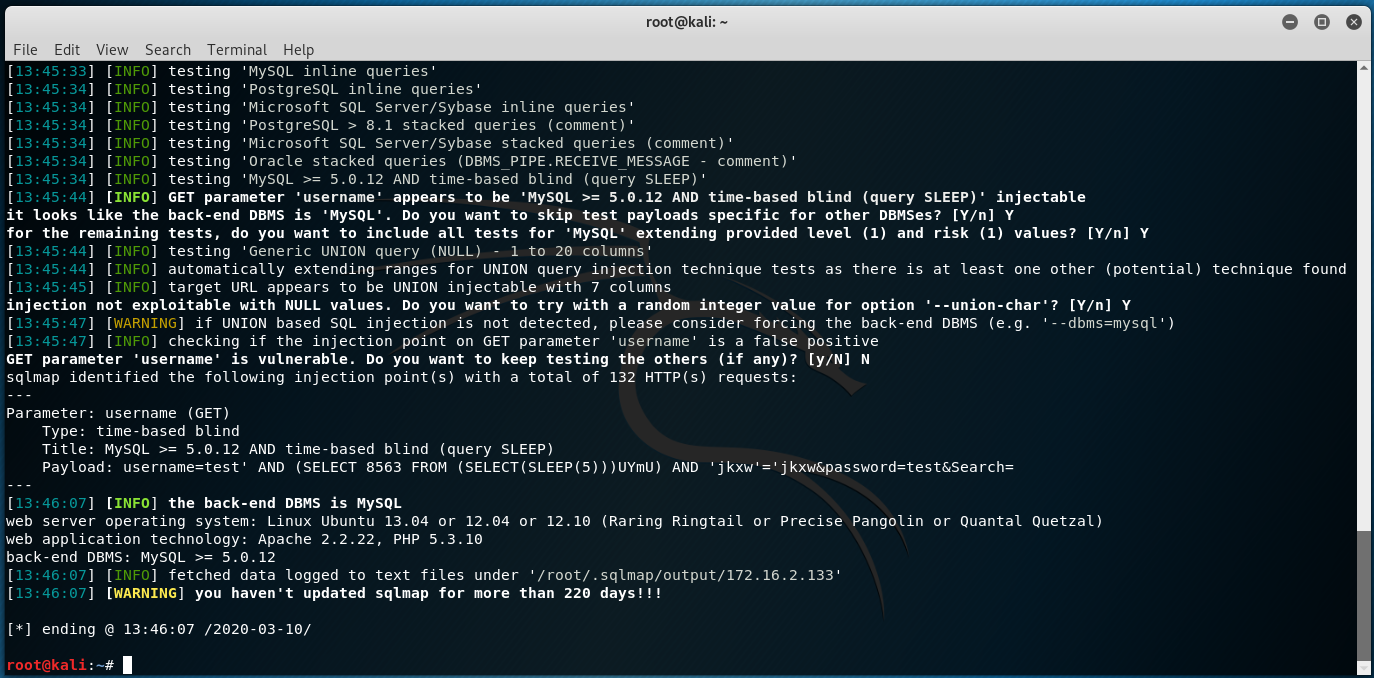
\includegraphics[scale=0.3]{img/sqlmap1.png}
	\caption{Initial SQLmap testing}
\end{figure}	
\begin{figure}[!htb]
	\centering
	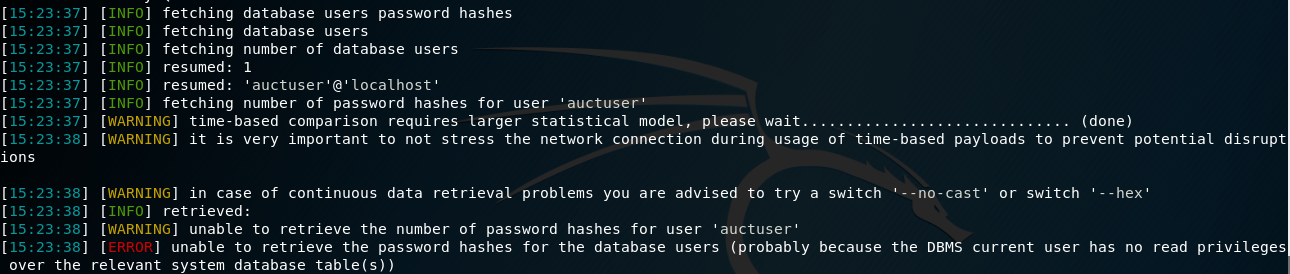
\includegraphics[scale=0.4]{img/sqlmap1.5.png}
	\caption{Finding DB users}
\end{figure}
\begin{figure}[!htb]
	\centering
	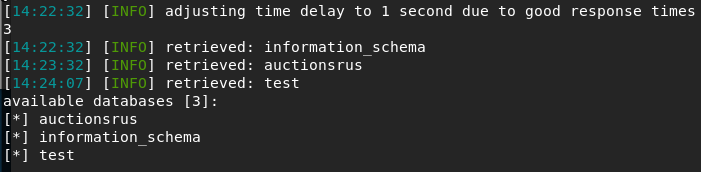
\includegraphics[scale=0.6]{img/sqlmap2.png}
	\caption{Finding DB names}
\end{figure}
\begin{figure}[!htb]
	\centering
	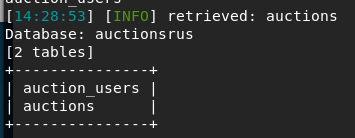
\includegraphics[scale=0.7]{img/sqlmap3.png}
	\caption{Finding table names}
\end{figure}
\begin{figure}[!htb]
	\centering
	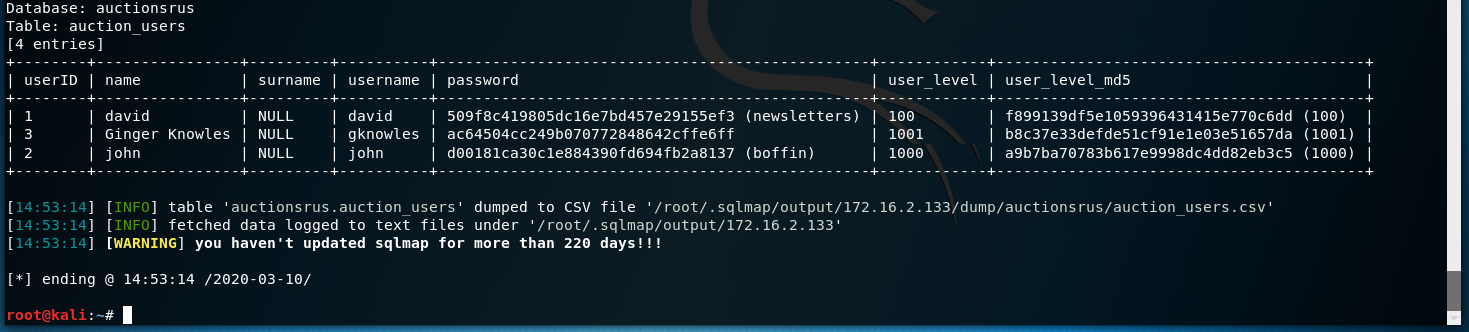
\includegraphics[scale=0.4]{img/sqlmap4.png}
	\caption{Dumping user data}
\end{figure}
\pagebreak



\subsection{Weak Authentication}
\subsubsection{Security Implications / Risk Level}
Weak authentication is another blanket term for a multitude of security vulnerabilities surrounding the authentication systems on a website. Again, these exploits can manifest in a number of forms, and have varying levels of risk depending on the exploit.\\
During testing a number of vulnerabilities were found that could be classed under weak authentication. These were:
\begin{itemize}
	\item Susceptibility to bruteforce attacks: There appeared to be no rate-limiting or IP blocking functionality on the website login form, allowing for bruteforce attacks to be performed easily. These attacks could potentially result in user accounts being accessed by attackers.
	\item Weakly hashed passwords: Using SQLmap, the users table was dumped, revealing that the passwords were hashed with unsalted MD5. This is a very weak algorithm, allowing it to be cracked quickly, as well as it having a plethora of rainbow tables already available online. This could result in hackers easily cracking passwords if they were able to retrieve the hashes.
	\item Weak session IDs: Instead of a secure session ID, the session IDs used within the website are simply an MD5 hash of the user level for that account. This is extremely dangerous, as an attacker can easily enumerate through the user levels, testing each one and gaining access to every account with ease.
\end{itemize}

\subsubsection{Cause of Vulnerability}
The exploits found each had varying causes, depending on which part of the website was being interacted with. These included:
\begin{itemize}
	\item Susceptibility to bruteforce attacks: The lack of a rate-limit or IP block on each account for the login form allows attackers to attempt as many times as they want, which makes bruteforce attacks possible. 
	\item Weakly hashed passwords: The use of the MD5 hashing algorithm results in weak hashing security, which stems from either legacy code (from when MD5 was stronger) or poor security choices during the design of the system.
	\item Weak session IDs: Again, this is another issue stemming from poor security choices during the design stage. Session IDs should be chosen as a completely random string, so hackers cannot collate multiple hashes and find patterns between them. Using unsalted MD5 as the hashing algorithm for this makes it even worse, as it is very easy to reverse engineer the original text from the hashes due to the nature of the user ID being numeric.
\end{itemize}

\subsubsection{Steps to Replicate}
Bruteforcing the login form
\begin{itemize}
	\item To bruteforce the login form, a custom python script was used (Appendix A). This script read in usernames from a 'usernames.txt' file, and passwords from a provided wordlist (in this case english top 10000 wordlist). For each username, the script iterated through the passwords, sending a GET request using the python 'requests' library. If the text 'User Account' was found in the response text, this would indicate a successful sign in and print the found credentials before moving on to the next username.
	Using the script successfully found the credentials for the admin user 'david' (Fig. 3.11), and could likely find the rest if a more extensive wordlist was used.	
\end{itemize}
Cracking the password hashes from SQLmap
\begin{itemize}
	\item The password hashes gained from SQLmap were unsalted MD5, so one of the first things to check would be an online rainbow table (a database of hashes and their corresponding plaintexts). In this case, the website 'Crackstation' was used to reverse all three hashes (Fig. 3.12).
\end{itemize}
Enumerating the session IDs
\begin{itemize}
	\item To enumerate the session IDs, another custom python script was created (Appendix B). 
\end{itemize}
\begin{figure}[!htb]
	\centering
	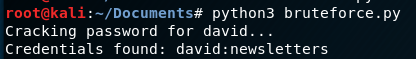
\includegraphics[scale=0.7]{img/bruteforce1.png}
	\caption{Bruteforcing the David user}
\end{figure}
\begin{figure}[!htb]
	\centering
	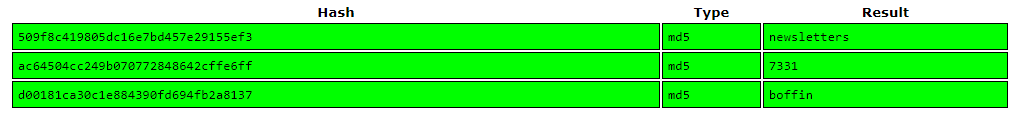
\includegraphics[scale=0.5]{img/crackstation.png}
	\caption{Cracking the hashes from SQLmap}
\end{figure}
\section{SRV1}
\section{SRV2}
\section{Ubuntu Client}

\chapter{Recommendations}
\section{Auction Site}
\section{SRV1}
\section{SRV2}
\section{Ubuntu Client}

\chapter{Conclusion}

\chapter{Appendices}
\section{Appendix A: Python bruteforce script}
\begin{figure}[!htb]
	\centering
	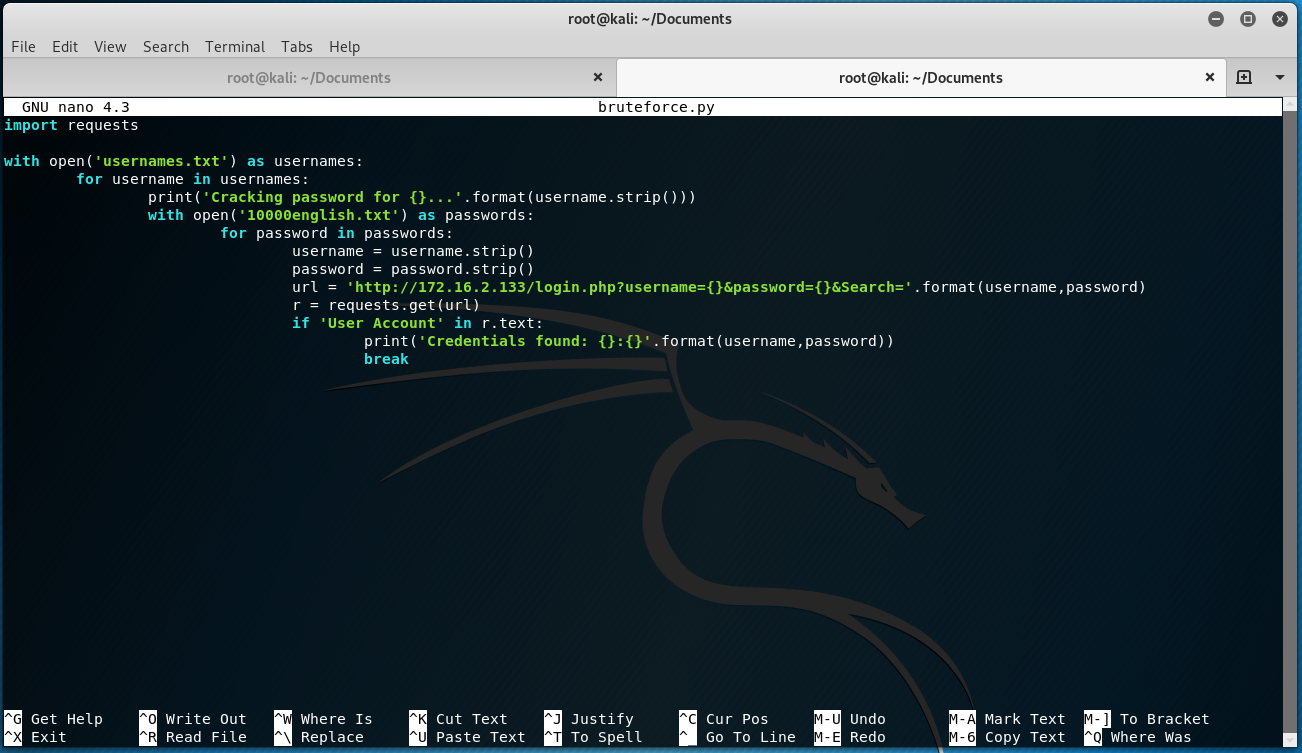
\includegraphics[scale=0.4]{img/bruteforcescript.png}
	\caption{Login form bruteforce script}
\end{figure}
\section{Appendix B: Session enumeration script}
\begin{figure}[!htb]
	\centering
	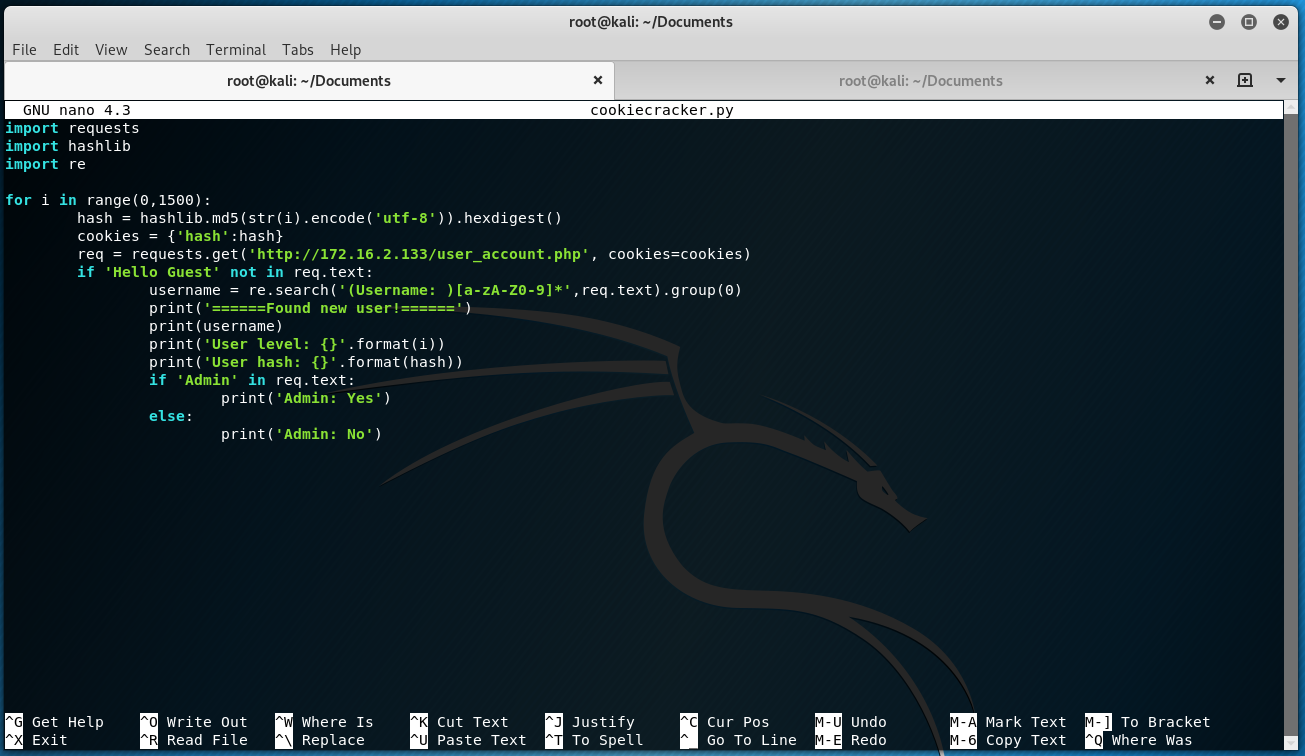
\includegraphics[scale=0.4]{img/cookiescript.png}
	\caption{Enumerating the session cookies}
\end{figure}

\chapter{References}


\end{document}